\subsection{Visual comparison}
\label{section:VisualComparison}
To decide if the results of the streaming implementation and the offline approach by \textcite{rakuschek2025visual} match they are are visually compared. To compare them one to one the window size $W$ is set to span the entire length of the input sequence. Normally streaming operations use smaller windows which discard historical observations to adapt to non stationary dynamics, nevertheless this causes the covariance matrix to represent recent observations rather then the global sequence of distribution. Additionally the online subspace iterations requires an decent number of sample updates to converge to an stable solution. Short sequences would compare the offline baseline against an non converged subspace estimate.\\
The evaluation is done on the datasets No.2 and No.30 with their corresponding descriptions found in \ref{app:dataset_description}. The time delay embedding parameters are set to a time lag of $/\tau = 1$ and embedding dimension of $d=15$, matching the reference setup. To force asymptotic convergence of the subspace iteration toward the true principal axes the algorithm executes multiple times successively over the input dataset.
\begin{figure}[H]
\centering
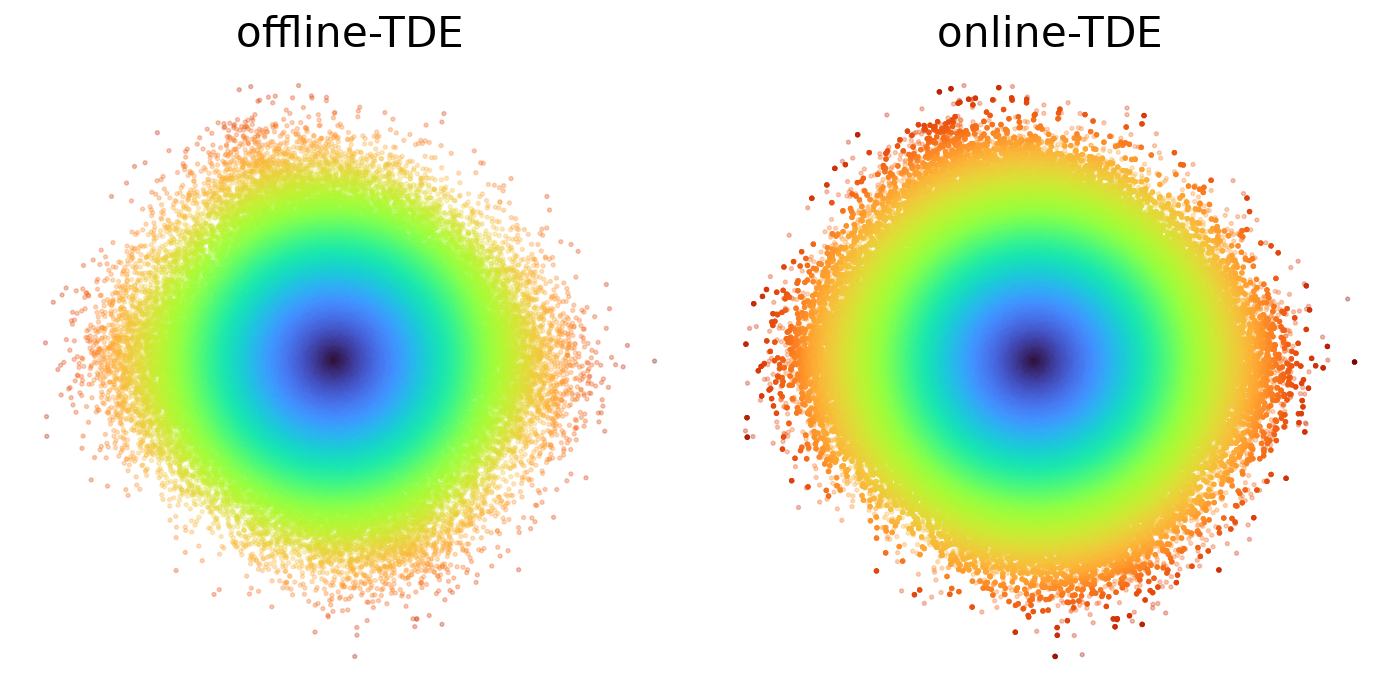
\includegraphics[width=1\textwidth]{figures/comparison_output_dataset2_d15_tau1_w102909.png}
\caption{Principle component analysis applied on dataset 02,with 102909 data points.}
\label{fig:tdeVisualComparison02}
\end{figure}
The plot generated from dataset 02 in figure \ref{fig:tdeVisualComparison02}(electric motor operating under healthy load and conditions) does not produce a distinct periodic shape in the projected subspace. The low amplitude vibrations characteristics of the normal operation  gather near the origin rather than forming a structured phase space geometry.
\begin{figure}[H]
\centering
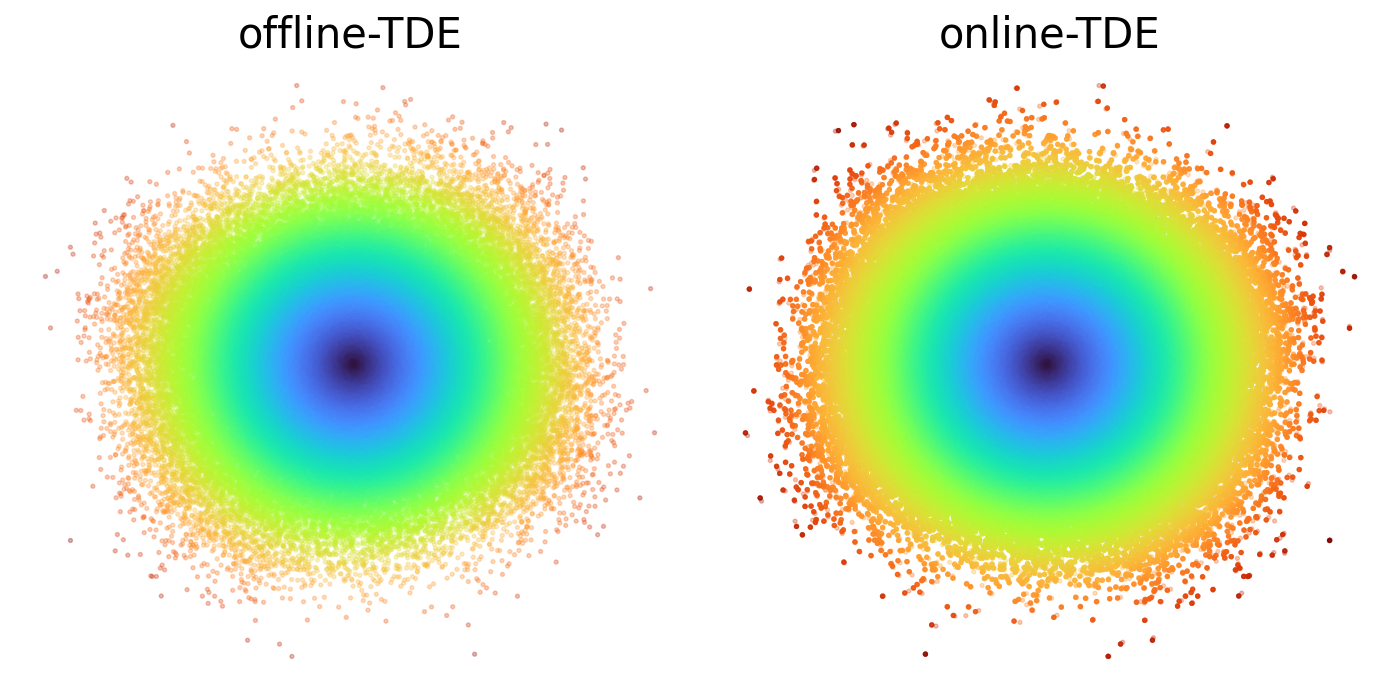
\includegraphics[width=1\textwidth]{figures/comparison_output_dataset30_d15_tau1_w101407.png}
\caption{Principle component analysis applied on dataset 30,with 102909 data points.}
\label{fig:tdeVisualComparison30}
\end{figure}
The comparison between the offline and online versions verifies that the streaming time delay embedding with principal component analysis and sliding windows produces correct values and generating visually identical structures.\\
Moreover this visual comparison produces an important insight regarding directly comparing "healthy" and "faulty" directly. Healthy states do not inherently produce clean  ellipsoid or ring like forms. As shown in Figure \ref{fig:tdeVisualComparison30},dataset 30(which contains mechanical faults with shaft misalignment) produces a significantly clearer continuous ring structure than the normal running condition Figure\ref{fig:tdeVisualComparison02}. This result emerges because high amplitude fault dynamics introduce strong harmonic components that forces the trajectory into phase space loops. This means diagnostic fingerprints cannot be evaluated by comparing an healthy and an faulty fingerprint next to each other. One solution would be to observe the phase space change over time which will be addresses in Section \ref{section:plotOverTime}